\chapter{Diseño y arquitectura del sistema}

\section{Estructura general}

El código del trabajo y todo lo que abarca se encuentra almacenando en \href{https://github.com/orgs/vieites-tfg/repositories?type=source}{GitHub}. Se han creado los repositorios necesarios en una misma organización de GitHub.

Entre los repositorios creados se pueden encontrar:

\begin{itemize}
  \item \texttt{zoo}.

    Este es el repositorio principal. Se trata de un \textit{monorepo}, en el que se encuentra implementado todo el código necesario para la realización del trabajo. Dentro del repositorio se encuentran:
    \begin{itemize}
      \item La aplicación de prueba sobre la que se apoya el proyecto, y que da nombre al repositorio, debido a que se trata de una aplicación de gestión de un zoo.
      \item Los módulos de Dagger para realizar los ciclos de CI y CD.
      \item Otros archivos, como \textit{scripts} y archivos de configuración.
    \end{itemize}

  \item \texttt{helm-repository}.

    Este repositorio alberga las Charts de Helm que definen la estructura necesaria para desplegar la aplicación de prueba.

  \item \texttt{state}.

    Se trata del repositorio en el que se almacenan los valores que poblarán los recursos de Kubernetes, dependiendo del entorno en los que se despliegue la aplicación. Además, en este repositorio también existe una rama de despliegue, de la cual ArgoCD lee los manifiestos de los recursos que debe desplegar para cada uno de los entornos.
\end{itemize}

En la figura~\ref{fig:ghorg} se muestra un diagrama de la disposición de los repositorios y la relación entre ellos.

\begin{figure}
  \centerline{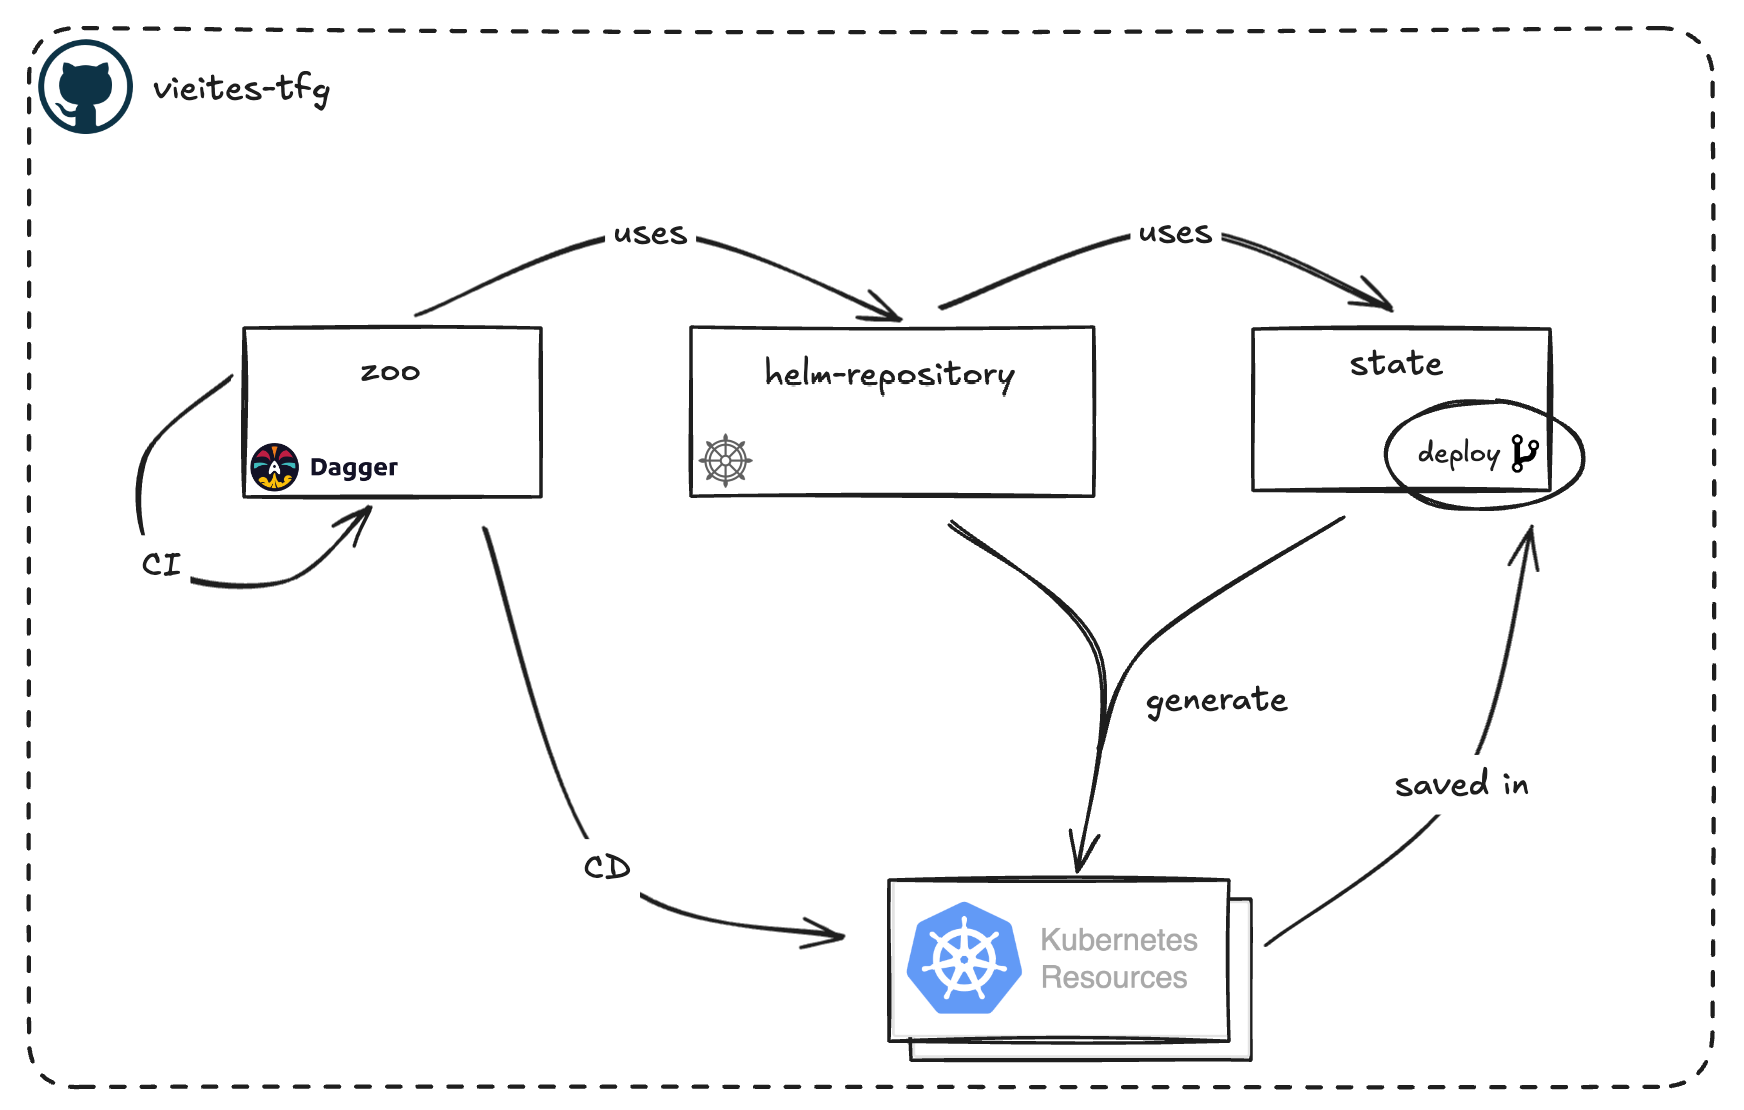
\includegraphics[width=14cm]{figuras/vieites-tfg}}
  \caption{Diagrama del la organización de GitHub. Imagen creada con \href{https://excalidraw.com}{excalidraw.com}}
  \label{fig:ghorg}
\end{figure}

\section*{zoo}

Como se ha comentado anteriormente, el repositorio \texttt{zoo} está estructurado como un \textit{monorepo}. Un \textit{monorepo} es un repositorio con diferentes proyectos, los cuales se encuentran interrelacionados de una manera bien definida. A lo largo de esta sección se justifica la elección de este tipo de estructura, a la vez que se explica cómo están implementados las diferentes piezas de software.

\subsection*{Aplicación de prueba}

\begin{figure}
  \centerline{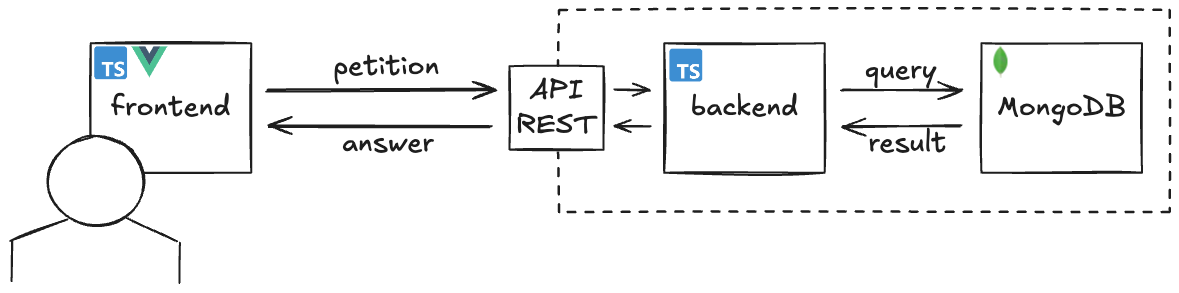
\includegraphics[width=15cm]{figuras/app}}
  \caption{Comunicación entre paquetes de la aplicación. Imagen creada con \href{https://excalidraw.com}{excalidraw.com}}
  \label{fig:app}
\end{figure}

La primera razón para escoger este tipo de estructura es el hecho de querer crear una aplicación relativamente pequeña, una página web que consta de un \textit{frontend} y un \textit{backend} (se hará referencia a estos como ``paquetes'' a partir de ahora). Por lo tanto, se hace más sencillo gestionar estos dos paquetes si viven juntos en un único repositorio.

Otra ventaja de utilizar un \textit{monorepo} tiene que ver con el software utilizado para crear los paquetes de la aplicación de prueba. Ambos se implementan utilizando Node.js, en lenguaje Typescript\cite{ts}. Los paquetes tienen dependencias propias, y se puede dar el caso de que ambos utilicen una o varias dependencias iguales. Usar un \textit{monorepo} permite tener esas dependencias en un mismo lugar, evitando su duplicado. Con esto se consigue reducir el tiempo de construcción de los paquetes.

Sin embargo, es necesaria una herramienta que permita manejar los paquetes de manera independiente. Alguno de los motivos para tener esta preferencia pueden ser: que haya dos equipos de desarrolladores, uno para cada paquete; o que se quiera publicar versiones, hacer tests, u otro tipo de tarea sobre cada paquete por separado. La herramienta que se utiliza en este trabajo se llama Lerna\cite{lerna}. Este software está específicamente diseñado para gestionar \textit{monorepos} de proyectos de Node.js. Entre las ventajas que proporciona se encuentran:

\begin{itemize}
  \item Gestión de tareas locales.
  \item Cacheo local de salidas de comandos, con posibilidad de dicha caché sea compartida entre entornos, por ejemplo, con agentes de CI.
  \item Detección de paquetes afectados por cambios en el código.
  \item Análisis de la estructura del proyecto.
\end{itemize}

Por los beneficios anteriormente comentados, y más, es por lo que se ha elegido esta herramienta para gestionar el \textit{monorepo}.

En cuanto a las tecnologías que se utilizan en la aplicación, ya se ha mencionado Typescript como lenguaje principal. Este lenguaje permite tener un sistema tipado, lo cual puede ser útil para detectar muchos errores comunes mediante el análisis estático en tiempo de construcción. Esto reduce las posibilidades de errores en tiempo de ejecución.

El \textit{backend} está completamente desarrollado utilizando dicho lenguaje. Su funcionalidad es proporcionar una API REST que el \textit{frontend} pueda utilizar para realizar cambios en la base de datos. Se usa MongoDB\cite{mongodb} como base de datos debido a que es fácil de gestionar y porque solo se almacena información sobre animales, sin ningún tipo de relación entre ellos, en una única tabla o documento.

El \textit{frontend} se ha implementado utilizando Vue.js\cite{vue}, un \textit{framework} que permite construir interfaces web mediante componentes reactivos. Se ha escogido este frente a otras opciones debido a su facilidad de uso sin conocimiento previo. Tiene una API intuitiva, por lo que no tiene una gran curva de apendizaje. Además, el propio \textit{framework} está construido utilizando Typescript, por lo que tiene compatibilidad de primera clase con este lenguaje.

En la figura \ref{fig:app} se puede ver un diagrama que muestra cómo es la comunicación entre los paquetes de la aplicación, y con la base de datos, junto con las tecnologías que se utiliza en cada uno de ellos.

\subsection*{Módulos de Dagger}

Se integran también en el repositorio los módulos de Dagger de CI y de CD. Estos módulos se incluyen en el \textit{monorepo} para facilitar la referencia a los paquetes que constituyen la aplicación de prueba. Además, tiene sentido que vivan en el mismo lugar una aplicación y las herramientas que permiten su evolución, como son cualquier tipo de software que realice las funciones de CI y de CD.

Ambos módulos se realizan utilizando el SDK del lenguaje Go que proporciona Dagger. Se ha escogido este lenguaje debido al conocimiento previo que ya se tenía de este. Además, es el lenguaje en el que está implementado el propio Dagger.

Uno de los módulos se encarga del ciclo de CI, es decir, de realizar los tests de la aplicación, del \textit{linting} o análisis del código en sí, y dela publicación de imágenes de Docker y paquetes NPM. Está organizado de manera que se pueden gestionar cada uno de los paquetes de la aplicación de manera independiente. Esto también es posible gracias al uso de Lerna, que ya se ha comentado anteriormente.

El segundo de los módulos, el de CD, realiza la tarea de publicación de los recursos de Kubernetes, los cuales son posteriormente obtenidos por ArgoCD para su despliegue completo. Esto se consigue haciendo uso de los repositorios \texttt{helm-repository} y \texttt{state}, en los cuales se almacenan las Charts de Helm y los valores que pueblan dichas Charts, respectivamente.

Se detalla más profundamente su implementación en el capítulo \ref{chap:dagger}.

\subsection*{Creación y configuración de los \textit{clusters}}
\label{subsec:clusters}

La fase final del ciclo de una aplicación es el despliegue. En este trabajo se levantan tres \textit{clusters} de KinD de manera local. Estos son los lugares en los que se despliega la aplicación. Generalmente se tienen diferentes \textit{clusters} con el fin de probar la aplicación en entornos distintos antes de desplegarla en el principal, que sería el de producción. El hecho de crearlos todos localmente hace que sean más sencillas las pruebas relacionadas con el despliegue. En equipos de desarrollo reales, los entornos de producción se encuentran en la nube. Sin embargo, sí que se pueden llegar a tener entornos locales para realizar pruebas de la aplicación.

Los \textit{clusters} se crean con el \textit{script} que se muestra en el Listing \ref{lst:create-clusters}. Este \textit{script} está escrito para funcionar en sistemas UNIX, en Bash, por lo que es un requisito utilizar un sistema operativo como MacOS o una distribución de Linux. No funcionará en un sistema operativo Windows. Se han puesto comentarios en vez de código algunas partes para reducir su tamaño, a modo de pseudocódigo. Estos son los pasos que se siguen para crear cada uno de los \textit{clusters}:

\begin{lstlisting}[language=bash,label=lst:create-clusters]{Script de creación de los clusters}
# Variables globales
# ---

for ENV in "${ENVS[@]}"; do
  case "${ENV}" in
    dev)
      BANNER_TEXT="We are in DEV";;
    # ... otros entornos
  esac

  CONTEXT="kind-${ENV}"

  kind create cluster --config "${CLUSTER_DIR}/kind_${ENV}.yaml"

  kubectl apply -f "${INGRESS_MANIFEST}" --context "${CONTEXT}"
  # Se espera a que se construya

  kubectl create namespace argocd || true

  cat "${SOPS_DIR}/age.agekey" |
    kubectl create secret generic sops-age -n argocd \
    --context ${CONTEXT} --from-file=keys.txt=/dev/stdin

  # Se descarga el repositorio de la Chart
  helm install argocd argo/argo-cd -n argocd \
    -f argo/values.yaml \
    # ... otros *flags*

  # Se espera a que se instale la Chart de Argo

  kubectl apply -f "${ARGO_DIR}/argo_${ENV}.yaml" \
    --context "${CONTEXT}"
  # Se espera a que se apliquen los cambios

  # Se aplica el banner a la interfaz de Argo

  # Se obtiene la clave inicial del usuario "admin" y se muestra
  # por pantalla
  PASSWORDS+="${current_pass}"
done

printf "${PASSWORDS}"
\end{lstlisting}

\begin{enumerate}
  \item Se indica el banner que va a tener cada uno de los \textit{clusters} (líneas 5-9).
  \item Se indica el contexto actual (línea 11), lo cual identifica cada \textit{cluster}. Esto es necesario a la hora de ejecutar comandos con \texttt{kubectl}, para asegurarse de que se está ejecutando cada comando sobre el \textit{cluster} que se precisa.
  \item Se crea el \textit{cluster} con su configuración específica (línea 13). Se puede ver el archivo de configuración del \textit{cluster} de \texttt{dev} en el Listing \ref{lst:conf-cluster}. Los archivos de los demás entornos son iguales a este, solo difieren en los puertos que se utilizan.
\begin{lstlisting}[language=helm,label=lst:conf-cluster]{Configuración del cluster de dev}
kind: Cluster
apiVersion: kind.x-k8s.io/v1alpha4
name: dev
networking:
  apiServerPort: 6443
nodes:
- role: control-plane
  kubeadmConfigPatches:
  - |
    kind: InitConfiguration
    nodeRegistration:
      kubeletExtraArgs:
        node-labels: "ingress-ready=true"
  extraPortMappings:
  - containerPort: 80
    hostPort: 8080
    protocol: TCP
  - containerPort: 443
    hostPort: 8443
    protocol: TCP
\end{lstlisting}
  \item Se instala el controlador de Ingress (líneas 15-16), lo cual permitirá acceder a la aplicación a través de una URL customizada desde el exterior.
  \item Se crea el \textit{namespace} en el que se va a instalar la instancia de ArgoCD (línea 18).
  \item Se crea un secreto en el que se almacena el valor de la clave de cifrado de los secretos de Kubernetes (líneas 20-22). El proceso de creación de cifrado y descifrado se explica en
    \begin{bclogo}[logo=\bcattention]{Important!}
      CITAR APARTADO EN EL QUE SE HABLA DE SOPS
    \end{bclogo}
  \item Se instala la Chart de Helm de Argo y se espera a que esté disponible (líneas 24-29). A la Chart se le pasan una serie de valores, de los cuales se habla en \ref{subsec:secretos}. Una vez instalado, se podrá acceder a ArgoCD de manera local. Para ello será necesario crear un ``túnel'' de un puerto libre local al puerto 443 del servicio principal de Argo. Esto se explica también en el
    \begin{bclogo}[logo=\bcattention]{Important!}
      CITAR MANUAL DE USUARIO
    \end{bclogo}
  \item Se aplica la configuración específica de Argo para el entorno que se está creando (líneas 31-33). Se puede ver la configuración para Argo en el entorno de \texttt{dev} en el Listing \ref{lst:conf-argo}. Lo más importante de esta configuración se encuentra en las líneas 9-11, en las cuales se indica el repositorio (\texttt{repoURL}), la ruta desde la raíz (el directorio \texttt{dev}) y la rama (\texttt{targetRevision}) de donde Argo debe obtener los archivos que definen recursos que se van a desplegar.
\begin{lstlisting}[language=helm,label=lst:conf-argo]{Configuración de Argo en dev}
apiVersion: argoproj.io/v1alpha1
kind: Application
metadata:
  name: app-dev
  namespace: argocd
spec:
  project: default
  source:
    repoURL: 'https://github.com/vieites-tfg/state.git'
    path: dev
    targetRevision: deploy
  destination:
    server: 'https://kubernetes.default.svc'
    namespace: dev
  syncPolicy:
    automated:
      prune: true
      selfHeal: true
    syncOptions:
      - CreateNamespace=true
\end{lstlisting}
  \item Se modifica el ConfigMap de Argo para que muestre el banner en la interfaz (línea 35).
  \item Se comprueba la contraseña inicial que tiene el usuario \texttt{admin} y se muestra por pantalla (líneas 37-39). Estas son las credenciales que hay que utilizar para poder hacer \textit{log in} en la interfaz de Argo. Por lo tanto, se muestran directamente por pantalla a medida que se van creando los \textit{clusters} y tras la creación de todos ellos (línea 42).
\end{enumerate}

En la figura \ref{fig:clusters} se puede observar cómo se sincroniza ArgoCD, en cada uno de los \textit{clusters}, con el repositorio de estado. Argo reacciona cada vez que se realizan cambios en el directorio que le corresponde, dentro de la rama de despliegue del repositorio \texttt{state}. En ese momento, obtiene de nuevo todos los archivos de definición de los recursos y se sincroniza con el estado deseado.

\begin{figure}
  \centerline{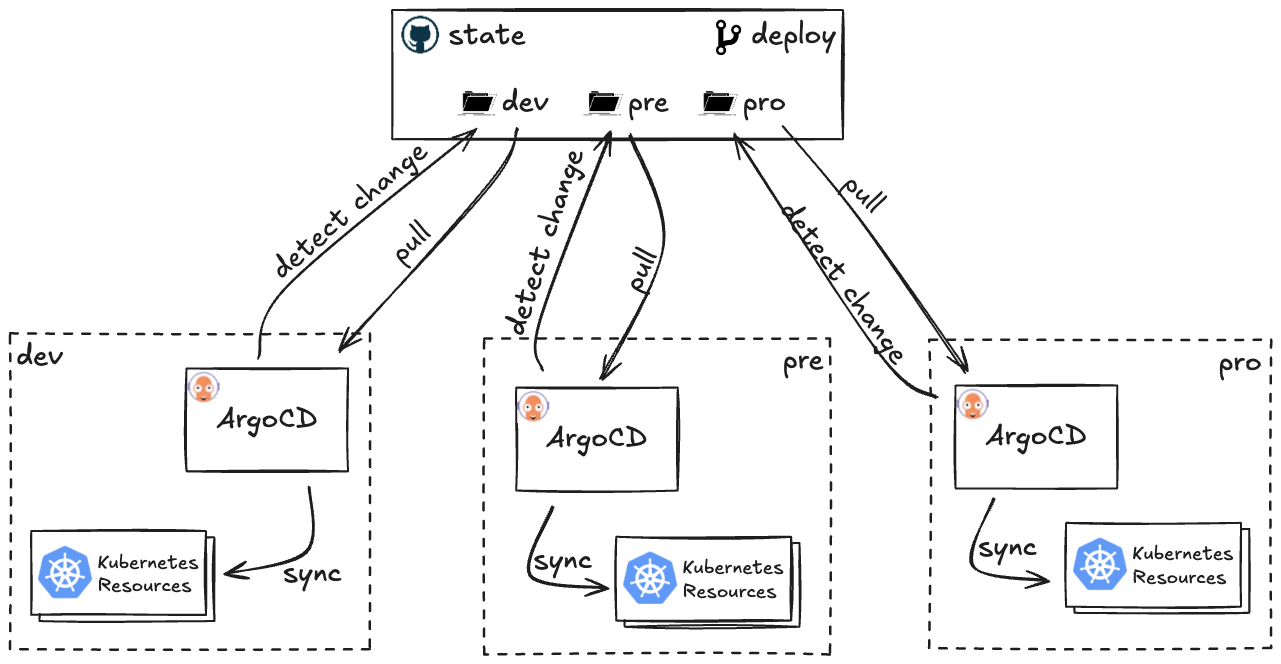
\includegraphics[width=15cm]{figuras/clusters}}
  \caption{Clusters y comunicación con el repositorio de estado. Imagen creada con \href{https://excalidraw.com}{excalidraw.com}}
  \label{fig:clusters}
\end{figure}

\subsection*{Gestión de secretos}
\label{subsec:secretos}

La aplicación de prueba consta de una base de datos, la cual tiene usuario y contraseña. Este es un ejemplo de datos que es necesario almacenar como un secreto o Secret de Kubernetes. Debido a que se está utilizando un método \textit{pull}\cite{pull} de despliegue de la aplicación; es decir, la herramienta que realiza el despliegue, ArgoCD, tira (hace \textit{pull}) del repositorio que le indicamos como objetivo; es necesario almacenar en el repositorio los secretos encriptados previamente. Esto es una buena práctica para evitar que se filtren sin querer los datos al exterior, aunque el repositorio sea privado.

Para encriptar los secretos se utilizan dos herramientas:

\begin{itemize}
  \item \texttt{age}\cite{age}.

    \texttt{age} es una herramienta creada con Go que permite encriptar y desencriptar archivos. Una vez instalada, es necesario crear unas claves privada y pública. Estas se proporcionan en el manual de usuario
    \begin{bclogo}[logo=\bcattention]{Important!}
      CITAR MANUALES DE USUARIO
    \end{bclogo}
    para poder probar la aplicación.
  \item SOPS\cite{sops}.

    SOPS (\textit{Secrets OPerationS}) permite editar archivos encriptados, pero con la capacidad de realizar la encriptación de campos específicos de tipos de archivos como YAML o JSON. Esta herramienta tiene compatibilidad con \texttt{age}, por lo que es un recurso excelente para encriptar recursos de Kubernetes, ya que estos se definen mediante archivos en formato YAML.

    El archivo de configuración de SOPS es como el que se muestra en el Listing \ref{lst:sops}. En él se indican: el formato de los nombres de los archivos que tiene que encriptar (línea 2), los campos que \textit{no} tiene que encriptar (línea 3) y la herramienta de encriptado junto con la clave pública que le sirve para realizar la encriptación (línea 4).

\begin{lstlisting}[language=helm,label=lst:sops]{Archivo de configuración de SOPS}
creation_rules:
  - path_regex: ".*\\.ya?ml$"
    unencrypted_regex: "^(apiVersion|metadata|kind|type)$"
    age: age15peyc7 #...
\end{lstlisting}

\end{itemize}

Con las claves pública y privada, y la configuración de SOPS, se es capaz de encriptar los Secrets de Kubernetes durante el ciclo de CD, en el módulo de Dagger. Los archivos encriptados se suben a la rama de despliegue del repositorio de estado, junto con los demás recursos que definen la aplicación.

Para desencriptar los secretos, ArgoCD necesita información: la clave privada creada con \texttt{age} y las herramientas necesarias para gestionar archivos encriptados con SOPS. La clave se le proporciona durante uno de los pasos de la creación de los \textit{clusters} \ref{subsec:clusters}. Sin embargo, es necesario decirle a Argo cómo utilizarla.

Para ello es necesario el uso de otras dos herramientas:

\begin{itemize}
  \item \texttt{kustomize}\cite{kustomize}.

    \texttt{kustomize} permite modificar valores de definiciones de recursos de Kubernetes sin necesidad de realizar cambios directamente en el archivo original, o bien crear recursos completamente nuevos a partir de otros. Las customizaciones se definen igual que cualquier otro recurso de Kubernetes, como se muestra en el Listing \ref{lst:kustomization}. En dicho archivo, el cual se debe llamar \texttt{kustomization.yaml}, se indican: \texttt{resources}, que son los archivos que se van a incluir tal y como estén definidos; y \texttt{generators}, archivos que muestran cómo construir recursos a partir de otros. El generador que se utiliza en este trabajo se muestra en el Listing \ref{lst:generator}. Estos archivos los lee ArgoCD, los interpreta, y así sabe cómo comportarse y las herramientas que tiene que utilizar cuando encuentra los archivos que definen los recursos, como \texttt{secrets.yaml} y \texttt{non-secrets.yaml}.

\begin{lstlisting}[language=helm,label=lst:kustomization]{Archivo 'kustomization.yaml'}
apiVersion: kustomize.config.k8s.io/v1beta1
kind: Kustomization
resources:
  - non-secrets.yaml
generators:
  - secret_generator.yaml
\end{lstlisting}

  \item \texttt{ksops}\cite{ksops}.

    \texttt{ksops} (kustomize-SOPS) es un \textit{plugin} de \texttt{kustomize} para gestionar recursos encriptados con SOPS. Se utiliza, sobre todo, para desencriptar Secrets o ConfigMaps de Kubernetes encriptados con SOPS. En el generador \ref{lst:generator} se ve cómo se le indica a ArgoCD que debe utilizar el \textit{plugin}  \texttt{ksops} para desencriptar el archivo con el nombre \texttt{secrets.yaml}.

\begin{lstlisting}[language=helm,label=lst:generator]{Generador de los secretos}
apiVersion: viaduct.ai/v1
kind: ksops
metadata:
  name: secret-generator
  annotations:
    config.kubernetes.io/function: |
      exec:
        path: ksops
files:
  - secrets.yaml
\end{lstlisting}

\end{itemize}

Lo único que falta es instalar dentro de Argo estas herramientas, \texttt{kustomize} y \texttt{ksops}, e indicarle dónde se encuentra la clave privada que usará para desencriptar los secretos.

Esto se consigue con los valores que muestran en la línea 26 del Listing \ref{lst:create-clusters}. El archivo \texttt{values.yaml} tiene el contenido que se muestra en el Listing \ref{lst:argo-values}. Con estos valores se consigue:

\begin{itemize}
  \item Indicar las \textit{flags} que tiene que utilizar Argo a la hora de ejecutar comandos con \texttt{kustomize} (líneas 1-4).
  \item Crear variables de entorno que informan (de arriba a abajo, respectivamente) el directorio raíz de archivos de configuración del sistema y la ruta en la que se puede encontrar la clave privada de \texttt{age} (líneas 6-11).
  \item Construir dos volúmenes, uno para almacenar los binarios de \texttt{kustomize} y \texttt{ksops}, y otro para la clave privada que se ha introducido en el \textit{cluster} en las líneas 20-22 del Listing \ref{lst:create-clusters} (líneas 13-18).
  \item Instalar los binarios de \texttt{kustomize} y \texttt{ksops} en el volumen \texttt{custom-tools} creado previamente (líneas 20-21).
  \item Permitir a Argo acceder a los binarios y a la clave, montando los volúmenes que contienen estos elementos dentro del servidor principal de Argo (líneas 33-41).
\end{itemize}

\begin{lstlisting}[language=helm,label=lst:argo-values]{Valores que pueblan la Chart de ArgoCD}
configs:
  cm:
    kustomize.buildOptions: "--enable-alpha-plugins --enable-exec"
    ui.bannerpermanent: "true"

repoServer:
  env:
    - name: XDG_CONFIG_HOME
      value: /.config
    - name: SOPS_AGE_KEY_FILE
      value: /.config/sops/age/keys.txt

  volumes:
    - name: custom-tools
      emptyDir: {}
    - name: sops-age
      secret:
        secretName: sops-age

  initContainers:
    - name: install-ksops
      image: viaductoss/ksops:v4
      command: ["/bin/sh", "-c"]
      args:
        - echo "Installing KSOPS and Kustomize...";
          mv ksops /custom-tools/;
          mv kustomize /custom-tools/;
          echo "Done.";
      volumeMounts:
        - mountPath: /custom-tools
          name: custom-tools

  volumeMounts:
    - mountPath: /usr/local/bin/kustomize
      name: custom-tools
      subPath: kustomize
    - mountPath: /usr/local/bin/ksops
      name: custom-tools
      subPath: ksops
    - name: sops-age
      mountPath: /.config/sops/age
\end{lstlisting}

Los archivos: \texttt{kustomization.yaml}, \texttt{secret\_generator.yaml}, \texttt{secrets.yaml} y \texttt{non-secrets.yaml}; todos ellos son los ficheros que se disponen en la rama de despliegue \texttt{deploy} del repositorio \texttt{state}. Por lo tanto, son los archivos que ArgoCD obtiene y utiliza para desplegar toda la aplicación en los distintos entornos.

En la figura \ref{fig:secrets} se puede ver el ciclo completo de encriptado y desencriptado de secretos

\begin{figure}
  \centerline{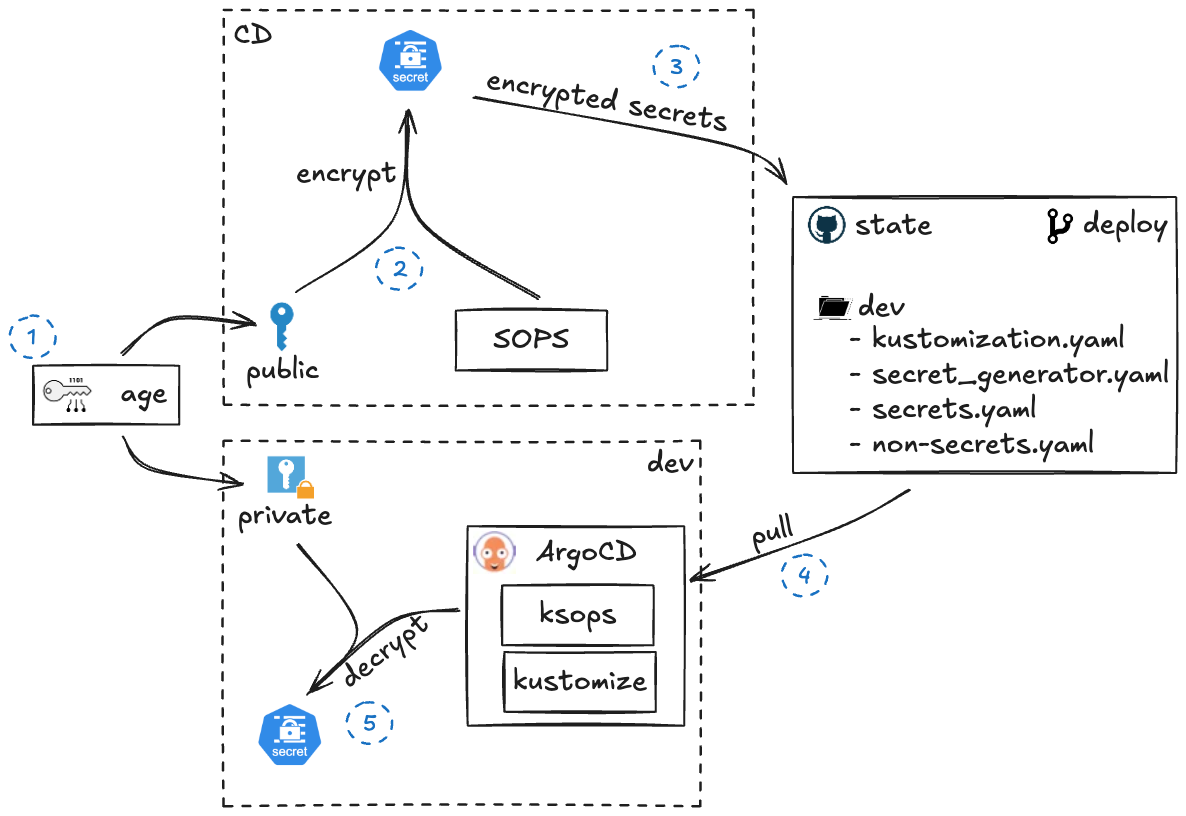
\includegraphics[width=13.5cm]{figuras/secrets}}
  \caption{Clusters y comunicación con el repositorio de estado. Imagen creada con \href{https://excalidraw.com}{excalidraw.com}}
  \label{fig:secrets}
\end{figure}

\subsection*{Función de cada \textit{cluster} y promoción de entornos}

A continuación se explica para qué se utiliza cada \textit{cluster} y cuál es el proceso de despliegue de la aplicación en cada uno de los entornos.

\begin{itemize}
  \item \texttt{dev}.

    Se trata del \textit{cluster} de desarrollo. En este se despliega la aplicación en el momento en el que se añade una nueva funcionalidad, ya sea en el \textit{frontend} o en el \textit{backend}. Esto implica, en términos de GitHub:

    \begin{enumerate}
      \item Crear una \textit{Pull Request} (PR) en la que se implementa la nueva funcionalidad. Esta debe ser siempre lo más reducida posible, cumpliendo con la filosofía de CI. Esto implica que la intención del equipo de desarrollo debe ser desplegar nuevas funcionalidades o correcciones de errores en producción en el menor tiempo posible. Se puede conseguir esto planeando PRs cortas en cuanto a tiempo de desarrollo, evitando que el equipo tenga demasiado trabajo en progreso y asignando los recursos necesarios para que cada PR se lleve a cabo lo más rápidamente\cite{linear}.
      \item Implementar la funcionalidad o realizar la corrección pertinente. A medida que se implementa, se puede, y es una buena práctica, ejecutar localmente el ciclo de CI para asegurarnos de que se pasan las pruebas y el \textit{linting} del código. Esta es una de las ventajas principales de utilizar Dagger. El desarrollador puede comprobar de manera local si el código actualizado es capaz de pasar el \textit{pipeline} de CI, lo cual evita tener errores inesperados a la hora de integrar el código en la rama principal.
      \item Revisar que la tarea que correspondía hacer en dicha PR se ha realizado correctamente.
      \item Integrar la funcionalidad o corrección en la rama principal del repositorio.
    \end{enumerate}

    Tras haber terminado todos los pasos anteriores, se ejecuta un \textit{workflow} de GitHub que realiza todo el ciclo de CI y CD, independientemente del entorno en el que se vaya a desplegar. El workflow es el que se ve en el Listing \ref{lst:workflowcicd}. En este se realizan los siguientes pasos:

\begin{lstlisting}[language=workflows,label=lst:workflowcicd]{Workflow de CI/CD}
on:
  push:
    branches: [ main ]
  release:
    types: [ published ]
  workflow_dispatch:

jobs:
  cicd:
    runs-on: ubuntu-24.04
    steps:
      - % Clona el repositorio "zoo" en la ruta "/zoo"

      - % Clona el repositorio "state" en la ruta "/state"
        % utilizando el token STATE_REPO

      - name: Install Dagger
        uses: dagger/dagger-for-github@8.0.0

      - name: Determine environment
        id: env_tag
        run: |
          % Determina el entorno en el que se despliega, teniendo
          % en cuenta el *trigger* que ha lanzado el workflow:
          %   - *push*    -> main
          %   - *release* -> *release* o *pre-release*

          echo "environment=${envi}" >> "$GITHUB_OUTPUT"
          echo "tag=${tag}" >> "$GITHUB_OUTPUT"

      - name: Recreate needed files
        run: |
          % Recrea el archivo .env para tenerlo disponible en
          % "zoo"
          echo "CR_PAT=${{ secrets.CR_PAT }}" >> ./.env
          % .... se incluyen todas las variables

          % Almacena la clave privada de "age"
          % Crea el archivo de configuracion de SOPS

      - name: Run Dagger CI module
        run: |
          tag=${{ steps.env_tag.outputs.tag }} 

          update_state () {
            % Actualiza el valor en "state" de la *tag* de la
            % imagen para que se despliegue la que se acaba de
            % publicar
          }

          dagger call --sec-env=file://.env backend \
              publish-image --tag "${tag}"
          update_state "zoo-backend" "${tag}"

          dagger call --sec-env=file://.env frontend \
              publish-image --tag "${tag}"
          update_state "zoo-frontend" "${tag}"

      - name: Run Dagger CD module
        run: |
          dagger call -m "./dagger/cd" \
            --socket=/var/run/docker.sock \
            --kind-svc=tcp://localhost:3000 \
            --config-file=file://cluster/kind_local.yaml \
            deploy \
            --sec-env=file://.env \
            --env=${{ steps.env_tag.outputs.environment }} \
            --age-key=file://sops/age.agekey \
            --sops-config=file://sops/.sops.yaml
\end{lstlisting}

    \begin{enumerate}
      \item Se clonan los repositorios necesarios (líneas 12-15).
      \item Se instala Dagger (líneas 17-18).
      \item Se determina el entorno y la \textit{tag} que se le pondrá a la imagen de Docker de los paquetes de la aplicación (\textit{backend} y \textit{frontend}) (líneas 20-29). Esta \textit{tag} es diferente para cada entorno. En el entorno de \texttt{dev} se trata de los ocho primeros caracteres del último \textit{commit} que se ha realizado. De esta manera se sabe a ciencia cierta el código que conforma la aplicación en dicha imagen, y facilita la detección de errores. El entorno es \texttt{dev} siempre que el evento que haya disparado el \textit{workflow} sea un \textit{push} de la PR a la rama principal, en este caso \texttt{main}.
      \item Se recrean los archivos necesarios con las variables almacenadas en GitHub (líneas 31-39). Se proporcionan estos archivos y datos en los manuales de usuario
        \begin{bclogo}[logo=\bcattention]{Important!}
          CITAR MANUALES DE USUARIO
        \end{bclogo}
        para su testeo en local.
      \item Se ejecuta el ciclo de CI para ambos paquetes de la aplicación y se publica cada una de las imágenes, indicando la \textit{tag} que se ha determinado previamente (líneas 51-57). Además, es necesario actualizar los valores de las \textit{tags} en el repositorio de estado, el cual tiene un campo específico para indicar este dato (líneas 45-49).
        \begin{bclogo}[logo=\bcattention]{Important!}
          CITAR APARTADO EN EL QUE SE HABLA DE STATE
        \end{bclogo}
      \item Se ejecuta el ciclo de CD, aportando los parámetros necesarios, entre los que se encuentran los archivos que se han construido previamente (líneas 59-69).
    \end{enumerate}

    Finalmente, la instancia de ArgoCD instalada en el entorno se sincroniza con el repositorio, obtiene los recursos de Kubernetes que se han almacenado en este y despliega la aplicación.

  \item \texttt{pre}

    Este es el entorno de pre-producción. Este tipo de entornos están diseñados para simular el entorno de producción real, y funciona como prueba final previa a la publicación de una aplicación de manera pública. En el caso de este trabajo, como ya se ha comentado, todos los entornos son idénticos, pero en equipos y entornos reales, cada uno de ellos tiene características distintas.

    Diferencias con respecto al entorno de \texttt{dev}:

    \begin{itemize}
      \item Se publica la imagen y los recursos en este entorno siempre que el evento que lanza el \textit{workflow} sea la creación de una \textit{prerelease}.
      \item La \textit{tag} que se utiliza es la que se le pone al nombre de la \textit{prerelease}. Esta debería tener formato SemVer\cite{semver} con una coletilla \textit{snapshot} (e.j. \texttt{1.2.3-snapshot}. Se utiliza esta coletilla con el fin de dar a entender que dicha imagen es una copia o ``captura'' de lo que sería la versión final de la imagen, la que se publicaría en el entorno de producción.
    \end{itemize}

    Los pasos que se realizan en el \textit{workflow} son los mismos, solo cambian los elementos que se acaban de indicar.

  \item \texttt{pro}

    Finalmente, el entorno de producción. Aquí es donde se despliega la aplicación de manera abierta a los usuarios. Como se lleva insistiendo a lo largo de este capítulo, lo normal es que estos entornos se encuentren en la nube. Para facilidad de pruebas y debido a que no es la finalidad de este trabajo, se ha decidido crear todos los \textit{clusters} de forma local.

    Cambios en este entorno con respecto a los anteriores:

    \begin{itemize}
      \item Se despliega la aplicación en él cuando el evento que lanza el \textit{workflow} no es una \textit{prerelease}, sino una \textit{release}.
      \item Al igual que en \texttt{pre}, la \textit{tag} sigue el formato SemVer, pero en este caso sin la coletilla que se usaba antes (e.j. \texttt{1.2.3}).
    \end{itemize}

\end{itemize}

En la figura \ref{fig:promotion} se muestra cómo el \textit{workflow} escucha los diferentes eventos que hacen que se ejecute el ciclo de CI/CD. Dependiendo del evento que ocurre, se va a utilizar una \textit{tag} diferente y se va a desplegar entorno correspondiente (\texttt{env}).

\begin{figure}[h]
  \centerline{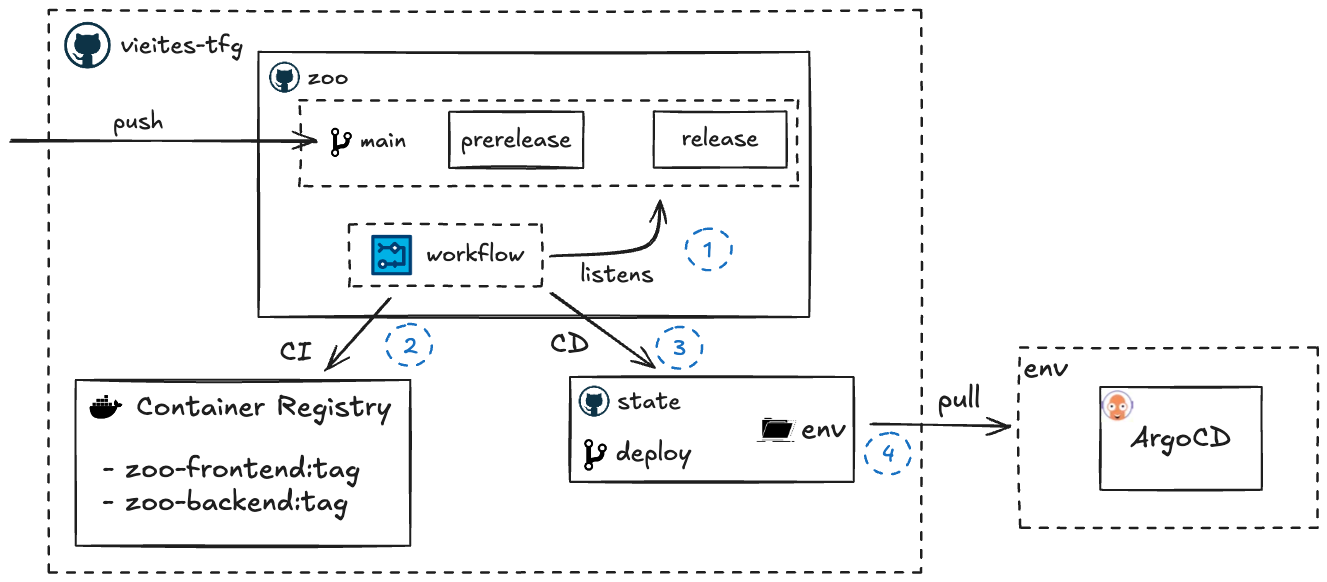
\includegraphics[width=13cm]{figuras/promotion}}
  \caption{Descripción del proceso de promoción de entornos. Imagen creada con \href{https://excalidraw.com}{excalidraw.com}}
  \label{fig:promotion}
\end{figure}

% Además, también se encuentran en este repositorio los módulos de Dagger de CI y de CD, y los \textit{scripts} y archivos de configuración necesarios para lanzar en local los \textit{clusters} de KinD que representan cada uno de los entornos en los que se despliega la aplicación. El hecho de que todo lo anterior se encuentre en un mismo repositorio hace mucho más sencilla su gestión.

% Debe describirse como se realiza o Sistema, a división deste en diferentes compoñentes e a comunicación entre eles. Así mesmo, determinarase o equipamento hardware e software necesario, xustificando a súa elección no caso de que non fose un requisito previo. Debe achegarse a un nivel suficiente de detalle que permita comprender a totalidade da estrutura do produto desenvolvido, utilizando no posible representacións gráficas.
